\documentclass[../main.tex]{subfiles}

\begin{document}
In a linear model, when the number of features is too large, we need to perform
some kind of feature selection to keep the benefits of the interpretability.
To do so, it is now common to penalize the problem.
Methods such as LASSO \citep{Tibshirani96} or Elastic-Net \citep{Zou_Hastie05}
use penalties to counteract different issues.
The $\ell_1$ penalty is used to induce some sparsity in the obtained estimation
and the $\ell_2$ penalty to take into account the correlation amongst the
features and regularize the data.

\medskip

With a dataset $X\in\bbR^{n\times p}$, the interactions matrix $Z$ has
$\cO(p^2)$ features, and thus quickly becomes very large.
This leads to solvers very time consuming in practice.
Since our problem has a specific architecture, we can use methods
that exploit it: like block optimization solvers.
We compare a Coordinate Descent with interactions \citep{Bascou_Lebre_Salmon20}
with Proximal Gradient Descent algorithms \citep{Beck17}.
We exploit the structure by block of the interaction matrix (\Cref{sec:CBPG})
to use the Cyclic Block Proximal Gradient method.

%%%%%%%%%%%%%%%%%%%%%%%%%%%%%%%%%%%%%%%
%% Notation
%%%%%%%%%%%%%%%%%%%%%%%%%%%%%%%%%%%%%%%

\section{Notations and reminders}

We denote $[k]=\{1, \dots, k\}$.
For any matrix $A$, $A_{ij}$ is its $(i,j)$-entry, $a_j$ the $j^{th}$ column.
For a subset $\mathcal{J} \subset [k]$, $A_{\mathcal{J}}$ is the sub-matrix
$(a_j)_{j\in \mathcal{J}}$ with $\#\mathcal{J}$ columns.
We use the same notation on a vector to consider the components of those indexes.
The $2$-norm $\norm{A}_2$ is the largest singular value of $A$ in magnitude.
For two vectors $u,v\in\bbR^k$, $(u\odot v)_i=u_iv_i$ is the
element-wise product. The $\ell_1$ norm is $\norm{u}_1=\sum_{j\in[k]}\abs{u_i}$,
and the squared $\ell_2$ norm is $\norm{u}_2^2 = \sum_{j\in[k]} u_j^2$.

\medskip

In the followings, we will consider our dataset the matrix
$X=[x_1|\dots| x_p]\in\bbR^{n\times p}$ the concatenation of the $p$ features.
Following the ideas from \citep{le2018whinter}, we use
$\tau_K : [p]^2 \longrightarrow [K]$ a function to index our interactions.
Meaning that in the interaction matrix $Z$, $Z_{\tau_K(i,j)} = x_i\odot x_j$.
In our situation, we have $K=q=\nicefrac{p(p+1)}{2}$.
And finally, we define the index of the block generated by $x_j$ as the branch
$\branch{K}{j}:=\{\tau_K(j,l),\ l\in [p]\}$.
So for example
\begin{align*}
Z_{\branch{q}{2}}=[x_2\odot x_2| \dots| x_2\odot x_p] \enspace.
\end{align*}

%%%%%%%%%%%%%%%%%%%%%%%%%%%%%%%%%%%%%%%
%% Explain the model and PGD procedure
%%%%%%%%%%%%%%%%%%%%%%%%%%%%%%%%%%%%%%%

\section{Presentation of the model}

For a dataset $X\in\bbR^{n\times p}$, the Elastic-Net estimator with first order
interactions $Z$ reads:
\begin{align} \label{pb:init} \tag{$\cP$}
	\widehat{p}
	& \in \min_{\substack{\beta \in \bbR^p \\ \Theta \in \bbR^q}}
		\frac{1}{2 n} \norm{y - X\beta - Z\Theta}^2_2 +
		\lambda_{\beta, \ell_1} \norm{\beta}_1 +
		\lambda_{\Theta, \ell_1}\norm{\Theta}_1 +
		\frac{\lambda_{\beta, \ell_2}}{2} \norm{\beta}_2^2 +
		\frac{\lambda_{\Theta, \ell_2}}{2} \norm{\Theta}_2^2 \\
	 & \in \min_{\substack{\beta \in \bbR^p \\ \Theta \in \bbR^q}}
		f(\beta, \Theta) +
		g^{(1)}_{\lambda_{\beta, \ell_1}, \lambda_{\beta, \ell_2}}(\beta) +
		g^{(2)}_{\lambda_{\Theta, \ell_1}, \lambda_{\Theta, \ell_2}}(\Theta)
		\enspace. \nonumber
\end{align}
Splitting the two penalty functions allow us to consider a gradient based
descent algorithm for the minimization, alternating the optimization on $\beta$
and $\Theta$.

\subsection{Optimization tools}

Since our objective to minimize is a convex non-differentiable function,
it is necessary for us to remind some mathematical tools.
In the following, the functions considered are proper (extended real function
that is not identically equal to $+\infty$ and cannot take the value $-\infty$).
They are also closed (their epigraph (see \Cref{def:epigraph}) is a closed set)
and convex.

\begin{definition}
	Let $f:\,\cX\rightarrow \bbR \cup \{+\infty\}$. The proximal operator of $f$
	evaluated at $u\in \cX$, denoted by $\prox_{\mu f}(u)$, with
	$\mu>0$ is defined as:
\begin{align}\label{def:prox}
	\prox_{\mu f}(u) =
	\argmin_{x\in\cX} \left\{ f(x) + \frac{1}{2\mu} \|x-u\|^2_2 \right\},
	\enspace.
\end{align}
\end{definition}

Proximal operators are essential in optimization methods. It is indeed possible
to show \citep[p.~270]{Beck17} that using a proximal operator to find the next
iterate in a problem to minimize formulated as a sum
is a generalization of solving a constrained-set objective minimization with
projected gradient method \citep{combettes2011proximal}.
Closely related to the proximal operators is the infimal convolution:

\begin{definition}\label{def:infconv}
	Let $f$ and $g$ two functions in $\bbR \cup \{+\infty\}$.
	Then the infimal convolution $f\square g$ is:
	\begin{equation}
		f\square g(x)
		= \inf_{u\in\cX} \left\{f(u) + g(x-u) \right\}\enspace.
	\end{equation}
\end{definition}

It is easy to see how the infimal convolution $f\square g$ is a regularization
of the function $f$ in the convex case by looking at
the epigraphs \citep{fajardo2012infimal}.
\begin{definition}\label{def:epigraph}
For a real function $f$ over $\cX$, the epigraph $\epi(f)$ is:
\[\epi(f)=\{(x, y)\in \cX\times \bbR\,|\, f(x)\leq y\}\enspace.\]
\end{definition}
The link with the infimal convolution is given thanks to the Minkowski sum.
As a reminder, the Minkowski sum of two sets of vectors $A$ and $B$ is:
$A\oplus B = \{a+b, a\in A, b\in B\}\enspace.$

\begin{proposition*}
    For two real functions $f$ and $g$:
    \begin{equation}\label{prop:epi}
    \epi(f\square g) = \epi(f)\oplus \epi(g)\enspace.
    \end{equation}
\end{proposition*}

Let us consider an example to visualize \Cref{prop:epi}.
For $x\in\bbR$, we take $f(x)=\abs{x}(1+\iota(\abs{x}\leq 1))$ and
$g(x)=\iota(0\leq x \leq 2)$, with $\iota$ the convex indicator function that
equals $0$ if the condition is met and $+\infty$ o.w.
Then
\begin{align*}
    f\square g(x)
	&= \min_{u\in\bbR} \{\abs{u} (1 + \iota (-1\leq u \leq 1))
	+ \iota(0\leq x-u\leq 2)\}
	\enspace.
\end{align*}

\begin{figure}[h!]
	\centering
	\begin{subfigure}{.4\textwidth}
		\centering
		\includegraphics[width = \textwidth]{f_g_infconv}
		\caption{Epigraphs of $f(x)=\abs{x}(1+\iota(\abs{x}\leq 1))$ and
		$g(x)=\iota(0\leq x \leq 2)$.}
	\end{subfigure}
	\begin{subfigure}{.4\textwidth}
		\centering
		\includegraphics[width = \textwidth]{f_g_infconv_minkowski}
		\caption{Epigraph of $f\square g(x)$.}
	\end{subfigure}
	\caption{Visualization that the epigraph of the infimal convolution is the
	Minkowski's sum of the epigraphs.}
\end{figure}

This implies that $f\square g(x)$ is not infinite for
$u\in [-1, 1]\cap [x-2, x]$ \ie for $x \in [-1, 3]$.
We can then decompose the problem:
\begin{itemize}
    \item if $x=-1$, then $u=-1$ and $f\square g(-1)=1$ and if $x=3$,
	then $u=1$ and $f\square g(1)=1$,
    \item if $x\in ]0, 2]$, then $f\square g(x) = 0$,
    \item if $x\in ]-1, 0]$ then $f\square g(x) = f(x)$,
    \item and finally if $x\in ]2, 3[$, then $u\in ]2-x, 1[$ and
	$f\square g(x) = \abs{2-x}$.
\end{itemize}

Taking in particular $g$ in \Cref{def:infconv} as
$g(u)=\frac{1}{2\mu}\norm{u}_2^2$ we obtain the Moreau envelope.

\begin{definition}
	For a function $f:\,\cX\rightarrow \bbR\cup\{+\infty\}$, the Moreau envelope
	is:
	\begin{align}
	\mathrm{M}_f^\mu(x)
	= \min_{u\in \cX} \left\{ f(u) + \frac{1}{2\mu}\norm{x-u}_2^2\right\},
	\quad \mu\geq 0\enspace.
	\end{align}
Note that the proximal operator is simply the solution to the Moreau
envelope.
And this envelope is simply a lower, regularized, version of the
function $f$.
Thus it can be rewritten:
	\begin{align}
	\mathrm{M}_f^\mu(x)
	= \left\{ u\in \cX,\ f(u) + \frac{1}{2\mu}\norm{x-u}_2^2
	= f\square \frac{1}{2\mu}\norm{\cdot}_2^2(x)\right\},
	\quad \mu\geq 0\enspace.
	\end{align}
\end{definition}
Moreau's envelope is the key of our minimization algorithms.
Indeed, it is equivalent to minimize $f$ or $\mathrm{M}_f^\mu$.
And it is possible to prove \citep[chapter 6]{Beck17} that
$\prox_{\mu f}(x) = x - \mu\nabla \mathrm{M}_f^\mu(x)$ which is simply a
gradient step to minimize $M_f^\mu$ and thus $f$.
Another key concept in optimization of non-differentiable functions
(such as the $\ell_1$ norm present in the Elastic-Net) is the subdifferential.
\begin{definition}
	Let $f:\,\cX\rightarrow \bbR\cup\{+\infty\}$ be a real convex function.
	Then the subdifferential $\partial f$ is:
	\begin{align}\label{def:subdif}
		\forall x\in\dom(f)\quad
		\partial f(x) = \left\{ f^* \in \cX^*,\ f(u) \geq f(x) +
		\langle f^*, u-x\rangle\ \forall u\in \cX\right\}
		\enspace.
	\end{align}
\end{definition}

For example, it is well known that the absolute function is not differentiable
at the origin. But as we can see in \Cref{fig:subgrad_abs},
\[\partial \abs{x} =
\begin{cases}
	-1, & \text{ if } x <0, \\
	1, & \text{ if }x>0, \\
	[-1, 1],& \text{ else }. \end{cases}
\]

\begin{figure}[h]
	\centering
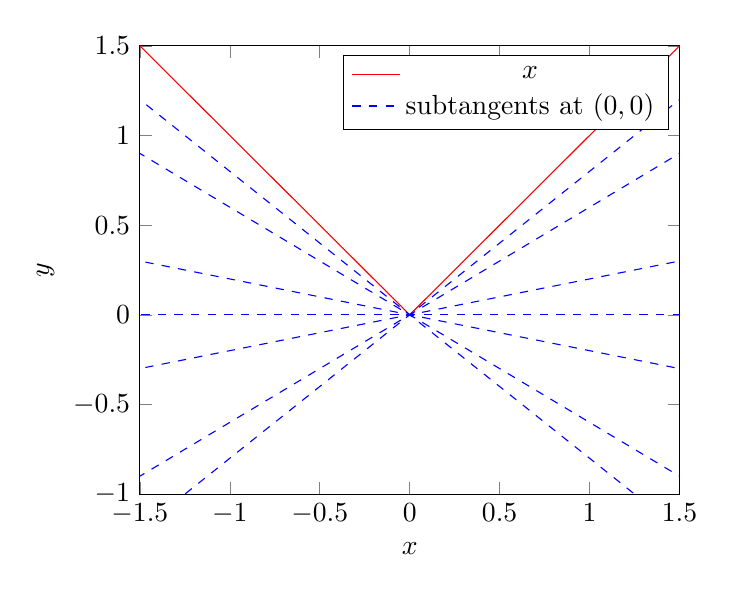
\begin{tikzpicture}[scale=1]
\begin{axis}[
		xlabel=$x$,
		ylabel=$y$,
		xmin=-1.5,   xmax=1.5,
		ymin=-1,   ymax=1.5,
	]
\addplot[mark = none, samples at={-1.5,0,1.5}, color=red]{abs(x)};
\addlegendentry{$\abs{x}$};
\foreach \fact in {-.8, -.6, -.2, 0, .2, .6, .8} {
	\addplot[dashed, mark = none, color=blue]{\fact*x};
	}
\addlegendentry{subtangents at $(0,0)$};
\end{axis}
\end{tikzpicture}
\caption{Visualization of the subtangents of the absolute value at $(0,0)$.
The slopes of the subtangents are in $\partial \abs{x}_{|_{x=0}}=[-1,1]$.}
\label{fig:subgrad_abs}
\end{figure}

\subsection{Coordinate descent algorithm for differentiable functions}

If we consider the minimization of a differentiable function $f$,
Coordinate Descent optimization is a possibility.

\begin{algorithm}[H]
	\caption{Coordinate Descent for a differentiable function $F$}
	\SetKwInOut{Input}{Input~}
	\SetKwInOut{Output}{Output~}
	\Input{$\eta>0$ step-size, $x=(x_i)_{i=1}^p$ initial vector,
	$\epsilon>0$ the tolerance}

	\While{stopping criterion $> \epsilon$}{
		\FOR{$i=1,\dots,p$}{
			$x_i \longleftarrow  x_i - \eta \dfrac{\partial F}{\partial x_i}(x)$
			}
			}
			\Output{$x_i$}
	\label{algo:Algo_CD}
\end{algorithm}

\Cref{algo:Algo_CD} performs a gradient descent step on each coordinate.
So instead of minimizing everything at once like we would with the gradient
descent update:
\begin{align}\label{eq:gd_step}
 \beta \longleftarrow \beta - \eta X^\top (X\beta - y) \enspace,
\end{align}
it reduced our problem of dimension $p$ to $p$ problems of dimension $1$.
This strategy for the steps direction is visible in \Cref{fig:cd_intuition}.
In practice, the step size used is the squared $\ell_2$ norm of each feature.
In the case of the least squares $\norm{y - X\beta}_2^2$,
with $X\in\bbR^{n\times p}$, we update the $i^{th}$ coordinate of $\beta$
with step $\eta>0$ using \Cref{eq:update_beta_cd}:
\begin{align}\label{eq:update_beta_cd}
	\beta_i \longleftarrow \beta_i - \eta x_i^\top (X\beta - y)\enspace.
\end{align}
As we will see in \Cref{sub:pgd_algo}, proximal operators allow us to minimize
our objective even if it is defined by an $\ell_1$ norm.
Meaning that the principle of Coordinate descent, which is minimizing each
coordinate, can be kept.

\medskip

Note that in Algorithm \ref{algo:Algo_CD} we chose to update the coordinates
cyclically.
Other strategies exist, such as a greedy implementation that will optimize
the coordinate with the largest decrease.
Some alternatives also use random choices for the updates \citep{nesterov2012efficiency}.
One important detail is about the residuals update.
\Cref{eq:update_beta_cd} uses the residuals $X\beta - y$ to update the coordinate.
Instead of recomputing the residuals from scratch at each step, it is more
efficient to see that between two iterates $\beta^{new}$ and $\beta^{old}$
for which $j_0$ is updated:
\begin{align*}
X\beta^{new} - y
& = X\beta^{old} - y - X_{j_0}\beta^{old}_{j_0} + X_{j_0} \beta^{new}_{j_0}
\enspace.
\end{align*}
So denoting $r^{old}$ and $r^{new}$ the residuals associated to $\beta^{old}$
and $\beta^{new}$, it follows that
\begin{align}\label{eq:resid_upd_cd}
	r^{new} = r^{old} - X_{j_0} (\beta^{old}_{j_0} - \beta^{new}_{j_0})
	\enspace.
\end{align}
By doing so, an update with Coordinate Descent is made of two operations
of complexity $\cO(n)$.

\subsection{Proximal Gradient Descent algorithms}\label{sub:pgd_algo}

Where Coordinate Descent minimizes each coordinate at a time, the idea
behind Proximal Gradient Descent is to minimize them all at once.
In a Least-Square problem with coefficients $\beta$ with a convex penalty function
$g$, the Proximal Gradient Descent algorithm is:

\begin{algorithm}[H]
	\caption{Proximal Gradient Descent for $X\in\bbR^{n\times p}$
	(regularized OLS)}
	\SetKwInOut{Input}{Input~}
	\SetKwInOut{Output}{Output~}
	\Input{$\beta=0_p$ initial vector, $\epsilon>0$ the tolerance}
	$L \longleftarrow \frac{\norm{X^\top X}_2}{n}$ \hspace{2cm} \textcolor{blue}{// step size (see \Cref{sec:step_size})}


	\While{stopping criterion $> \epsilon$}{
		\FOR{$i=1,\dots,$}{
			$\beta \longleftarrow  \prox_{\frac{1}{L}g}\left(\beta - \frac{1}{Ln} X^\top (X\beta - y)\right)$
			}
			}
	\Output{$\beta$}
	\label{algo:Algo_PGD}
\end{algorithm}

The convergence rate is of course slower.
However exploiting the architecture of the problem and using the GPU can
make Proximal Gradient Descent based methods competitive.
One important difference in the computation is for the residuals.
Since we update all coordinates at once, \Cref{eq:resid_upd_cd} will result in:
\begin{align}
	r^{new} = r^{old} - X(\beta^{old} - \beta^{new})\enspace,
\end{align}
resulting in one $\cO(np)$ operation.
\Cref{fig:cd_intuition} shows that instead of having steps performed
parallelly with the axes, we can advance in diagonals
(optimize multiple coordinates at once).
\begin{figure}[h]
	\centering
	\includegraphics[width=\textwidth]{cd_intuition}
	\caption{Path of the iterates of PGD and CD to minimize the cost function in a LASSO
	problem with a random matrix $n=200$ and $p=2$.}
	\label{fig:cd_intuition}
\end{figure}

\medskip

In our case, Problem \eqref{pb:init} is not to minimize a single function but a sum of
convex functions with two variables $\beta$ and $\Theta$.
Using Proximal Gradient Descent \citep{Beck17} in alternating setting,
we obtain the following iterates for the $k^{th}$ step
\begin{align}
	\beta^{k+1}  & =
	\prox_{\frac{1}{L_X}g^{(1)}}
	\left(\beta^k - \frac{1}{L_X}
	\frac{\partial}{\partial \beta}f(\beta^k, \Theta^k)
	\right)\enspace, \\
	\Theta^{k+1} & =
	\prox_{\frac{1}{L_Z}g^{(2)}}
	\left(\Theta^k - \frac{1}{L_Z}
	\frac{\partial}{\partial \Theta}f(\beta^{k+1}, \Theta^k)
	\right)\enspace,
\end{align}
where $L_X$ and $L_Z$ are Lipschitz constants for the partial derivatives
to be determined.
We still need to calculate the derivatives of $f$ \wrt each component.
Direct computation shows that:
\begin{align}
	\frac{\partial f}{\partial \beta}(\beta, \Theta)
	= \frac{1}{n}X^\top (X\beta + Z\Theta - y)
	\quad \text{and} \quad
	\frac{\partial f}{\partial \Theta}(\beta, \Theta)
	= \frac{1}{n}Z^\top (X\beta + Z\Theta -y)
	\enspace.
\end{align}
Now we can compute the Lipschitz constants.
For $L_X$, let $\beta_1,\beta_2\in\bbR^p$, we have
\begin{align*}
\norm{
	\frac{\partial}{
		\partial \beta}f(\beta_1, \Theta) -
		\frac{\partial}{\partial \beta}
		f(\beta_2, \Theta)}_2
	& = \frac{1}{n} \norm{ X^\top(X\beta_1 + Z\Theta - y) -
	 X^\top(X\beta_2 + Z\Theta - y) }_2 \\
	& = \frac{1}{n} \norm{ X^\top X\beta_1 - X^\top X\beta_2 }_2 \\
	& \leq \frac{1}{n} \norm{ X^\top X }_2 \norm{ \beta_1-\beta_2 }_2  \enspace.
\end{align*}
This bound is the smallest possible.
Let $L'>0$ be another Lipschitz constant.
Indeed, if we take $\beta_1$ the unit eigenvector associated to the largest
eigenvalue of $X^\top X$ and $\beta_2=0_p$ then:
\begin{align*}
\frac{\norm{X^\top X}_2}{n}
& = \frac{\norm{X^\top X\beta_1}_2}{n} \\
& = \frac{1}{n}\norm{X^\top X \beta_1 - X^\top X 0_p}_2 \\
& \leq L' \norm{\beta_1 - 0}_2 = L'
\enspace.
\end{align*}
We thus obtain that $L_X = \frac{\norm{ X^\top X }_2}{n}$
and with the same method $L_Z = \frac{\norm{ Z^\top Z }_2}{n}$.

%%%%%%%%%%%%%%%%%%%%%%%%%%%%%%%%%%%%%%%
%% Formulae for the prox operator
%%%%%%%%%%%%%%%%%%%%%%%%%%%%%%%%%%%%%%%

\section{Calculating the proximal operator}

With the Elastic-Net, the proximal operators allow us to minimize the objective
even though the penalty is not differentiable.
We now need to compute this operator.
For a function $h(x)=\|x\|_1 + \frac{\gamma}{2}\|x\|_2^2$, we know
\citep[p.~189]{Parikh14} that for $\mu>0$:
\[
\prox_{\mu h}(x) = \dfrac{1}{1 + \mu\gamma}\prox_{\mu \|\cdot\|_1}(x) =
\dfrac{\sign(x)}{1 + \mu\gamma}(|x| - \mu)_+\enspace,
\]
where $(\cdot)_+=\max(\cdot, 0)$.
With the penalty on $\beta$: $g^{(1)}$
(the second function $g^{(2)}$ is identical) we get
\begin{align}\label{par:proxi}
	\prox_{\mu g^{(1)}}(\beta) &
	= \prox_{\mu\lambda_{\beta, \ell_1}{h^{(1)}}}(\beta)
	= \dfrac{\sign(\beta)}{1 + \mu \lambda_{\beta,\ell_2}}(|\beta|
	-\mu\lambda_{\beta, \ell_1})_+\enspace,
\end{align}
with ${h^{(1)}}(\beta) = \|\beta\|_1 + \frac{\lambda_{\beta, \ell_2} /
 \lambda_{\beta, \ell_1}}{2} \|\beta\|_2^2$
such that $ \lambda_{\beta, \ell_1}{h^{(1)}}(\beta) = g^{(1)}(\beta)$.

\begin{definition}
We denote $\mathrm{ST}$ the soft-tresholding operator such that:

\[\mathrm{ST}(x, \lambda) = \sign(x)(|x| - \lambda)_+ = \begin{cases} x- \lambda & \text{ if } x>\lambda,\\
										  x + \lambda & \text { if } x < -\lambda,\\
										  0 & \text{ else }. \end{cases}
										  \]

\begin{figure}[ht]
	\centering
\begin{tikzpicture}[>=stealth', scale=1,]
	\tkzInit[xmin=-5,xmax=5,
			 ymin=-5,ymax=5,
			 xstep=2,ystep=2]
	% \tkzAxeXY[orig=false]
	\tkzLabelY[orig=false]
	\tkzLabelX
	\tkzDrawX
	\tkzDrawY
	\tkzFct[domain=-5:5,color=blue,very thick]{\x}
	\node[above] at (2,2.5) {$y=x$};
	\tkzFct[domain=2:5,color=red,very thick]{\x-2}
	\tkzFct[domain=-5:-2,color=red,very thick]{\x + 2}
	\tkzFct[domain=-2:2,color=red,very thick]{0}
	\node[above] at (-2,.5) {$y=\mathrm{ST}(x, 2)$};
	\end{tikzpicture}
	\caption{Soft-thresholding applied with $\lambda=2$.}
\end{figure}
\end{definition}

Updating $\beta$ thus leads to:
\begin{align}
	\beta^{k+1} = \frac{1}{1 +
	\frac{n}{\norm{ X^\top X}_2} \lambda_{\beta, \ell_2}}
	\mathrm{ST}
	\left( \beta^k - \frac{n}{\norm{ X^\top X}}
		\frac{1}{n} X^\top (X\beta^{k} + Z\Theta^k - y),
		\frac{n}{\norm{ X^\top X}_2}\lambda_{\beta, \ell_1}
	\right) \enspace.
\end{align}
For the update on $\Theta$, considering
\begin{align*}
u = \Theta^k - \frac{n}{\norm{ Z^\top Z}} \frac{1}{n} Z^\top (X\beta^{k+1} + Z\Theta^k - y)
\enspace,
\end{align*}
the gradient step associated, is then:
\begin{equation}
	\Theta^{k+1} = \frac{1}{1 + \frac{n}{\norm{ Z^\top Z}_2}
	\lambda_{\Theta, \ell_2}}\mathrm{ST}
	\left(
		u, \frac{n}{\norm{ Z^\top Z}_2}\lambda_{\Theta, \ell_1}
	\right) \enspace.
\end{equation}

%%%%%%%%%%%%%%%%%%%%%%%%%%%%%%%%%%%%%%%
%% CBPG
%%%%%%%%%%%%%%%%%%%%%%%%%%%%%%%%%%%%%%%

\section{Cyclic Block Proximal Gradient (CBPG)} \label{sec:CBPG}

With the Proximal Gradient Descent, we update all of the coordinates of
 $\beta$ and $\Theta$ at once.
With Coordinate Descent with interactions \citep{Bascou_Lebre_Salmon20}, in each
epoch we update each coordinate separately.
Some kind of compromise between the two algorithms is possible using the block
structure of the interaction matrix.
Indeed, we can do block updates of $\Theta$ separately using the
CBPG method \citep{massias2019sparse,Beck17}.
Doing so, we need the expression of the derivative involved for
each block and the associated Lipschitz constants.
Both can be retrieved using the same method as before, so we get:
\begin{align}
	&\frac{\partial}{\partial \Theta_{\branch{q}{i}}}f(\beta, \Theta)
	= \frac{1}{n} Z_{\branch{q}{i}}^\top (X\beta + Z\Theta - y)\enspace,\\
	&\norm{\frac{\partial}{\partial \Theta_{\branch{q}{i}}}
		f(\beta, \Theta_1) - \frac{\partial}{\partial \Theta_{\branch{q}{i}}}
		f(\beta, \Theta_2)}_2
	\leq \frac{1}{n}\bnorm{Z_{\branch{q}{i}}^\top Z}_2
		\bnorm{\Theta_1 - \Theta_2}_2\enspace.
\end{align}

We denote $L_i=\frac{1}{n}\norm{Z_{\branch{q}{i}}^\top Z}_2$ the Lipschitz
constant associated to the update of the $i^{th}$ block.
Notice that the residuals needed in the gradient can be updated by block as
in \Cref{eq:resid_upd_cd} to reduce the complexity.

\begin{algorithm}[H]
\label{algo:Algorithm_blockupdate}
\caption{Cyclic block proximal gradient for one epoch at iteration $k\geq 1$}
\SetKwInOut{Input}{Input~}
\SetKwInOut{Output}{Output~}
\Input{$X\in \bbR^{n\times p}$, $y\in\bbR^{n}$}

$\beta^{k+1} =  \prox_{\frac{1}{L_X}g^{(1)}}\left(
	\beta^k - \frac{1}{L_X}\frac{\partial}{\partial \beta}f(\beta^k, \Theta^k)
	\right)$,

\FOR{$i=1,\dots,p$}{
	$ \Theta^{k+1}_{\branch{q}{i}}= \prox_{\frac{1}{L_i}g^{(2)}}\left(
		\Theta^k_{\branch{q}{i}} -
		\frac{1}{L_i}\frac{\partial}{
			\partial \Theta_{\branch{q}{i}}}f(\beta^{k+1}, \Theta^k)\right)$
}

\Output{$\beta, \Theta$}
\end{algorithm}

%%%%%%%%%%%%%%%%%%%%%%%%%%%%%%%%%%%%%%%
%% Stopping criterion (to move smw later)
%%%%%%%%%%%%%%%%%%%%%%%%%%%%%%%%%%%%%%%
\section{Stopping criterion}

Finding a stopping criterion for iterative solvers is not a trivial task.
Necessary conditions for a point to be optimal exist such as the
Karush-Kuhn-Tucker (KKT) conditions.
For an objective $f$ penalized with $m>0$ inequality constraints
$h_i,\ i=1,\dots,m$ the minimization problem writes:
\begin{align*}
	\min_{x} f(x)\ s.t.\ h_i(x)\leq 0,\ i=1,\dots,m\enspace.
\end{align*}
This can be rewritten as minimizing the following Lagrangian function with
$\mu_1,\dots,\mu_m\in \bbR$:
\begin{align*}
	\cL(x, \mu_1,\dots,\mu_m) = f(x) + \sum_{i=1}^m \mu_i h_i(x)
	\enspace.
\end{align*}

\begin{proposition}
	The KKT conditions state that at the optimum $x^*$
	\begin{enumerate}
		\item $0\in \partial f(x^*) + \sum_{i=1}^m \mu_i \partial h_i(x^*)$
		(stationarity),
		\item $\forall i\in [m],\ \mu_i h_i(x^*)=0$ (complementary slackness),
		\item $\forall i\in [m],\ \mu_i>0$ and $h_i(x^*) \leq 0$ (feasibility).
	\end{enumerate}
\end{proposition}

To stop our solvers, we can look at how much we violate these conditions.
Simplifying the lines hereafter, let us consider an Elastic-Net problem
with $W\in\bbR^{n\times p}$:
\begin{align}\tag{$\mathcal{P}_{enet}$}
	\argmin_{w\in\bbR^p}
	\frac{1}{2n} \|y - Ww\|^2_2 + \lambda_1 \|w\|_1 +
	\frac{\lambda_2}{2}\|w\|^2_2 = \argmin F_{enet}(w)
	\enspace.
\end{align}
KKT conditions dictate that at the optimum $w^*$:
\begin{align*}
	0 \in W^\top (Ww^* - y) + \lambda_2 w^* + \lambda_1 \partial\norm{w^*}_1
	\enspace.
\end{align*}
For the primal $(\cP_{enet})$, we stop when current iterate $w$ is such that
$d_{\|\cdot\|}(0, \partial F_{enet}(w))\leq \epsilon$ for $\epsilon > 0$.
This means that we are at most violating the KKT conditions by $\epsilon$ for the
considered norm.
Since the subdifferential is a set, the distance considered is the distance of
a vector to a set.
For a vector $u\in\bbR^n$ and a set $E\subset \bbR^n$ it means:
\begin{align*}
	d_{\norm{\cdot}}(u, E) = \inf_{v\in E}\norm{u-v}\enspace.
\end{align*}
We will consider the $\infty$-norm to have all coordinates below $\epsilon$
in absolute value:
\begin{align}\label{eq:eps_kkt}
	\inf_{h\in \partial F_{enet}(w)} \|h\|_\infty\leq\epsilon\enspace.
\end{align}

We can consider the problem coordinate-wise as we will take the maximum over
the coordinates.
If $h\in\partial F_{enet}(w)$ then for $j\in [p]$,
\begin{align*}
	h_j \in \frac{1}{n} W_j^\top (W w - y) +
	\lambda_1 \partial_{|\cdot |}(w_j) + \lambda_2 w_j
	\enspace.
\end{align*}
The distance for each coordinate we want to compute is then:
\begin{align*}
	d(0, \partial F_{enet}(w)_j)
	&=
		d\left(0, \frac{1}{n}W_j^\top (Ww-y) +
		 \lambda_1\partial_{|\cdot |}(w_j)+\lambda_2w_j\right) \\
	&=
		d\left(-\frac{1}{n}W_j^\top(Ww-y) - \lambda_2w_j,
		\lambda_1\partial_{|\cdot |}(w_j)\right)\enspace.
\end{align*}
Denoting $r=y - Ww$ the residuals, we get:
\begin{align}
		d\left(\frac{1}{n} W_j^\top r - \lambda_2 w_j,
			\lambda_1\partial_{|\cdot|}(h_j) \right)
			&= \inf_{\eta_j \in \partial_{|\cdot|}(h_j)}
			\frac{1}{n} \left| W_j^\top r-n \lambda_2 w_j
				- n \lambda_1 \eta_j\right|
				\nonumber\\
			&= \frac{1}{n} \left| \mathrm{ST}\left( W_j^\top r - n \lambda_2 w_j
				,n\lambda_1 \right) \right| \enspace.  \label{eq:stop_coord}
\end{align}

We can stop the solver when the maximum value for $j\in[p]$ of
\Cref{eq:stop_coord} is below
$\epsilon$\footnote{see \Cref{chap:an_cv} for convergence rates results.}.
This strategy can be applied to our interaction problem considering that
$W = [X \,|\, Z]$ and $w=[\beta\,|\, \Theta]$.
\Cref{eq:stop_coord} then writes as:
\begin{align} \label{eq:stop_inter}
	d(0, \partial F_{enet}(w)_j)
			&= \frac{1}{n} \left| \mathrm{ST}\left( W_j^\top r - n
			 [\lambda_{\beta_, \ell_2} \mathds{1}(j \leq p) +
			 \lambda_{\Theta_, \ell_2} \mathds{1}(j > p)] w_j,
			 n[\lambda_{\beta_, \ell_1} \mathds{1}(j \leq p) +
			  \lambda_{\Theta_, \ell_1} \mathds{1}(j > p)] \right)
			  \right| \enspace.
\end{align}

\subsection{Reformulating the criterion from a LASSO perspective} \label{sub:equivLasso}

Since the Elastic-Net can be rewritten as a LASSO problem,
\Cref{eq:stop_coord} can also be derived from the KKT violation.
Indeed, we have:
\begin{align*}
	\frac{1}{2n}\norm{y-Ww}_2^2 + \lambda_1 \|w\|_1 +
								  \frac{\lambda_2}{2}\|w\|^2_2
	& = \frac{1}{2n}\norm{y-Ww}_2^2 + \lambda_1 \|w\|_1 +
         \sum_{j=1}^p\left(\frac{\sqrt{\lambda_2}}{2}w_j\right)^2 \\
	& = \frac{1}{2n}\left[\norm{y-Ww}_2^2 +
	    \sum_{j=1}^p\left(\sqrt{\lambda_2 n}w_j\right)^2\right]
		+ \lambda_1 \|w\|_1  \\
	& = \frac{1}{2n}\norm{\widetilde y - \widetilde Ww}_2^2
		+ \lambda_1 \|w\|_1
		\enspace,
\end{align*}
with $\widetilde W =
\begin{bmatrix} W \\
	 \sqrt{\lambda_2 n}\mathrm{Id}_{p\times p}
	\end{bmatrix} \in \bbR^{(n+p)\times p}$ and
$\widetilde y = [y \,|\, 0_p ]^\top\in\bbR^{(n+p)\times p}$.
\Cref{eq:eps_kkt} renders as:
\begin{align}
\max_{j\in [p]}  \frac{1}{n}
\left|\mathrm{ST}\left(\widetilde W_j^\top\widetilde r,
			 n\lambda_1 \right)\right|\leq \epsilon\enspace.
\end{align}
Working with interactions, Problem \eqref{pb:init} can be rewritten as
a weighted LASSO objective:
\[\min_{\beta, \Theta}\frac{1}{2n} \|\widetilde y -
		\widetilde X \beta - \widetilde Z\Theta\|_2^2 +
		\lambda_{\beta, \ell_1} \norm{\beta}_1 +
		\lambda_{\Theta, \ell_1} \norm{\Theta}_1\enspace,\]
with
\begin{align*}
	\widetilde y=[y\,|\, 0_p \,|\, 0_q]^\top \in \bbR^{n+p+q},
	\quad
	\widetilde X =
	\begin{bmatrix} X \\
		\sqrt{\lambda_{\beta, \ell_2} n}\mathrm{Id}_{p\times p}\\
		 0 \end{bmatrix}\in \bbR^{(n+p+q)\times p}
	\text{ and }
	\widetilde Z =
	\begin{bmatrix} Z \\
		 0 \\
		  \sqrt{\lambda_{\Theta, \ell_2} n}\mathrm{Id}_{q\times q}
		\end{bmatrix}\in\bbR^{(n+p+q)\times q}
		\enspace.
\end{align*}
To recover a weighted-LASSO, we concatenate both matrices.
We denote $\widetilde W = [\widetilde X \,|\, \widetilde Z]$,
$\widetilde w = [\beta \,|\, \Theta]$,
and $\lambda=[\lambda_{\beta, \ell_1}\mathbf{1}_p|
\lambda_{\Theta, \ell_1}\mathbf{1}_q]$, with $\mathbf{1}_p$ the vector of
ones of dimension $p$.
Problem \Cref{pb:init} renders as:
\[\argmin_{\widetilde w \in \bbR^{p+q}}
  \frac{1}{2n} \| y - \widetilde W \widetilde w\|_2^2
  + \sum_{j=1}^{p+q} \lambda_j \abs{\widetilde w_j}
  \enspace.\]
This leads to \Cref{eq:stop_inter} with a LASSO problem.
We can stop the solver when:
\[\max_{j\in [p+q]} \frac{1}{n} \left| \mathrm{ST}\left( \widetilde W_j^\top \widetilde r, n\lambda_j\right)\right|\leq \epsilon\enspace. \]

%%%%%%%%%%%%%%%%%%%%%%%%%%%%%%%%%%%%%%%%%%%%%%%%%%%%%%%%%%%%%%%
\section{Pipeline and discussion about the algorithm used}
%%%%%%%%%%%%%%%%%%%%%%%%%%%%%%%%%%%%%%%%%%%%%%%%%%%%%%%%%%%%%%%
\subsection{Main steps for the Cyclic Block pipeline}
%%%%%%%%%%%%%%%%%%%%%%%%%%%%%%%%%%%%%%%%%%%%%%%%%%%%%%%%%%%%%%%

Here, we synthetize the pipeline for the Cyclic Block Proximal Gradient
algorithm.
In \Cref{chap:an}, we will see how in practice we can use this algorithm,
especially the computation of the steps and how it performs on datasets.
%
\usetikzlibrary{arrows.meta}
\usetikzlibrary{positioning, calc}
\tikzset{%
  >={Latex[width=2mm,length=2mm]},
  % Specifications for style of nodes:
            base/.style = {rectangle, rounded corners, draw=black,
                           minimum width=4cm, minimum height=1cm,
                           text centered, font=\sffamily},
  activityStarts/.style = {base, fill=blue!30},
       startstop/.style = {base, fill=red!30},
    activityRuns/.style = {base, fill=green!30},
         process/.style = {base, minimum width=2.5cm, fill=orange!15,
                           font=\ttfamily},
}
\begin{figure}[ht]
\begin{tikzpicture}[node distance=1.5cm,
    every node/.style={fill=white, font=\sffamily}, align=center, scale=.7]

	\node (start) [activityStarts] {$X\in\bbR^{n\times p}$};
	\node (clone) [process, below left=.5cm of start] {
		Clone: $\widetilde{X} \leftarrow X$};
	\node (std) [process, below right=.5cm of start] {
		Standardize: $X\leftarrow \frac{X-\mu_X}{\sigma_X}$};
	\node (Z_std) [activityStarts, below of=clone]{
		Compute $\mu_Z$ and $\sigma_Z$ \\
		so $Z_{\branch{q}{j}}=\frac{\widetilde X_j \odot
		 \widetilde X_{\llbracket j,:\rrbracket} -
		 \mu_{Z_{\branch{q}{j}}}}{\sigma_{Z_{\branch{q}{j}}}}$};
	\node (Lip) [process, below of=std] {
		Apply algorithm \ref{algo:Lanczos} to compute:\\
		 $L_X$, $L_Z$ and $L_{Z_{\branch{q}{i}}}$, $i=1,\dots, p$};

	\draw[->] (start.west) [out=180, in=90] to (clone.north);
	\draw[->] (start.east) [out=-1, in=90] to (std.north);
	\draw[->] (std) -- (Lip);
	\draw[->] (Z_std) -- (Lip);
	\draw[->] (clone.east) [out=-5, in=10, looseness=2] to (Z_std.north east);

	\draw[red,thick,dotted] ($(start.north west)+(-6.5,0.6)$)  rectangle (
		$(Lip.south east)+(0.4,-0.6)$) node[above left]{preprocessing};

	\node (while) [activityRuns, below right=1cm of Z_std] {
		While KKT criterion $> \epsilon$};
	\node (beta) [process, below of=while] {PGD step to update $\beta$};
	\node (theta_i) [process, below of=beta] {
		Update each block of $\Theta$ consecutively.};

	\draw[->] (Z_std.south) -- (while.west);
	\draw[->] (Lip.south) -- (while.east);
	\draw[->] (while) -- (beta);
	\draw[->] (beta) -- (theta_i);

\end{tikzpicture}
\end{figure}

\medskip

The values in $\mu_X$, $\sigma_X$, $\mu_Z$ and $\sigma_Z$ can be stored once
and reused later by the solver.
So there we can also not clone the data at the beginning.
This implies keeping the non-standardized data during the run and
standardize on-the-fly when a matrix-vector product is computed.
The same applies to the Lipschitz constants that can be reused if different
regularizations are tested (like in a grid search).

\medskip

The cost of the KKT criterion is also very low because in \Cref{eq:stop_inter},
we only need the residuals.
Those are already computed so we do not need to recompute them.
So the most costly operations are the products with $X^\top$ and $Z^\top$
respectively in $\cO(np)$ and $\cO(nq)$.

\subsection{Discussion of using PGD/CBPG instead of CD}

As an example, we can consider the usual LASSO problem (as the Elastic-Net
is just an extension of the LASSO as we saw in \Cref{sub:equivLasso}).
We benchmark the convergence of the objective function
for CD and PGD methods, with and without acceleration in \Cref{fig:benchopt}.
\begin{figure}[h]
	\centering
	\includegraphics[scale=.7]{benchopt_plt}
	\caption{
		Suboptimality curves of CD and PGD to solve a simulated LASSO problem of
		$100$ samples and $5000$ features.
		We also compare with the solver from \texttt{Scikit-learn} (which is CD-based).
		The $\ell_1$ penalty is set to $0.1$.
		The parameter $\rho$ controls cross-correlations: for features $i$ and $j$,
		the cross-correlation is $C_{i,j} = \rho^{\abs{i-j}}$.
		Note that no GPU was used.
		}
		\label{fig:benchopt}
	\end{figure}

\Cref{fig:benchopt} was made with the \texttt{BenchOpt} library\protect\footnotemark.
As we can clearly see, PGD methods converge slowly, and even slower without
inertial acceleration.
Hereafter, the acceleration considered is Nesterov inertial acceleration
\citep{nesterov27method}.
This takes into account with a specific weight the previous iterate value.
\footnotetext{see \url{https://benchopt.github.io/} for the main page,
\url{https://benchopt.github.io/results} for the results visualization
(interactive with \texttt{Plotly}!) and \Cref{chap:benchopt} for more.}


\medskip

So trying to compete with CD is neither easy nor manageable with CPUs.
And if GPUs can, not necessarily beat CD, but only become a possible contestant,
then maybe other good statistical algorithms judged too time consuming could be
used again.
Not only old methods, new methods may be even faster using GPUs.

\end{document}